%% LaTeX-Beamer template for KIT design
%% by Erik Burger, Christian Hammer
%% title picture by Klaus Krogmann
%%
%% version 2.1
%%
%% mostly compatible to KIT corporate design v2.0
%% http://intranet.kit.edu/gestaltungsrichtlinien.php
%%
%% Problems, bugs and comments to
%% burger@kit.edu

\documentclass[18pt]{beamer}
\usepackage[utf8x]{inputenc}
\usepackage{units}
\usepackage{booktabs}

%% CUSTOM
\usepackage{amsmath}
\usepackage{algpseudocode}

%% Definitions
\DeclareMathOperator{\div2}{div}
\renewcommand{\algorithmicrequire}{\textbf{Input:}}
\renewcommand{\algorithmicensure}{\textbf{Output:}}
\algnewcommand\algorithmicto{\textbf{to}}
\algrenewtext{For}[3]{\algorithmicfor\ $#1 \gets #2$ \algorithmicto\ $#3$ \algorithmicdo}
\algnewcommand\algorithmicod{\textbf{od}}
\algrenewtext{EndWhile}{\algorithmicod}
\algrenewtext{EndFor}{\algorithmicod}
%\AtBeginSection[]{%
%\begin{frame}<beamer> % do nothing in handouts
%    \frametitle{Überblick}
%    \tableofcontents[sectionstyle=show/shaded,
%    subsectionstyle=show/show/hide]
%\end{frame}
%}
%\AtBeginSubsection[]{%
%\begin{frame}<beamer> % do nothing in handouts
%    \frametitle{Überblick}
%    \tableofcontents[sectionstyle=show/shaded,
%    subsectionstyle=show/shaded/hide]
%\end{frame}
%}

%% SLIDE FORMAT

% use 'beamerthemekit' for standard 4:3 ratio
% for widescreen slides (16:9), use 'beamerthemekitwide'

\usepackage{templates/beamerthemekit}
%\usepackage{templates/beamerthemekitwide}

 %% TITLE PICTURE

 % if a custom picture is to be used on the title page, copy it into the 'logos'
 % directory, in the line below, replace 'mypicture' with the 
 % filename (without extension) and uncomment the following line
 % (picture proportions: 63 : 20 for standard, 169 : 40 for wide
 % *.eps format if you use latex+dvips+ps2pdf, 
 % *.jpg/*.png/*.pdf if you use pdflatex)


 \titleimage{banner}
 
 
%% Define some colors:
\definecolor{darkblue}{rgb}{0,0,.5}
\definecolor{darkgreen}{rgb}{0,.5,0}

 %% TITLE LOGO

 % for a custom logo on the front page, copy your file into the 'logos'
 % directory, insert the filename in the line below and uncomment it

\titlelogo{logo_150x150}
 
 % (*.eps format if you use latex+dvips+ps2pdf,
 % *.jpg/*.png/*.pdf if you use pdflatex)
 
 %% TikZ INTEGRATION
 
 % use these packages for PCM symbols and UML classes
 % \usepackage{templates/tikzkit}
 % \usepackage{templates/tikzuml}
 
 % the presentation starts here
 
\author{Dominik Muth - dominik.muth@student.kit.edu}
\institute{Institut f\"ur Informatik}

\subtitle{Foliensatz 13}
\date{31. Januar 2013}

\newcommand{\sq}{$\square$}
\newcommand{\da}{$\downarrow$}
\DeclareMathOperator{\cod}{cod}

\begin{document}

\begin{frame}
    \titlepage
\end{frame}

\begin{frame}{Outline/Gliederung}
    \tableofcontents
\end{frame}

\section{Wiederholung}
\begin{frame}{Wiederholung}
    \begin{itemize}
        \item Was gehört zur formalen Definition einer Turingmaschine?\\
            \visible<2->{$T = \left( Z, z_0, X, f, g, m \right)$}
        \item Welche Eigenschaften haben Äquivalenzrelationen?
            \visible<3->{\begin{itemize}
                \item Reflexiv
                \item Symmetrisch
                \item Transitiv
            \end{itemize}}
        \item Und was heißt das?
    \end{itemize}
\end{frame}
\section{Unentscheidbare Probleme}
\begin{frame}{Unentscheidbare Probleme}
    Es gibt Probleme, die lassen sich mit einer Turing-Maschine (oder äquivalent: einem Java-Programm) nicht lösen. (Auch nicht mit unendlich viel Zeit und Platz.)\\
    Ein solches Problem ist nicht \emph{entscheidbar}
    \begin{block}{Entscheidbarkeit}
        Für ein entscheidbares Problem gibt es eine Turingmaschine, die für jede Eingabe hält und das Eingabewort entweder akzeptiert oder nicht.
    \end{block}
\end{frame}
\begin{frame}{Codierung von Turingmaschinen}
   Bisher haben wir eine Turingmaschine formal so geschrieben $T = \left( Z, Z_0, X, f, g, m \right)$. Wir bauen uns eine Codierung, die die ganze Turingmaschine in ein Wort $w_1$ ``packt''. \\
   \pause
   \begin{block}{Universelle Turingmaschine (UTM)}
       Dieses Wort $w_1$ übergeben wir dann einer universellen Turingmaschine $U$,
       \begin{itemize}
           \item die übeprüft, ob $w_1$ eine Turingmaschine $T$ codiert
           \item dann die Turingmaschine $T$ ``simuliert'' und als Eingabe $w_2$ verwendet
           \item und schließlich das Ergebnis davon ausgibt
       \end{itemize}
   \end{block}
   \visible<3->{\begin{figure}[h]
       \centering
       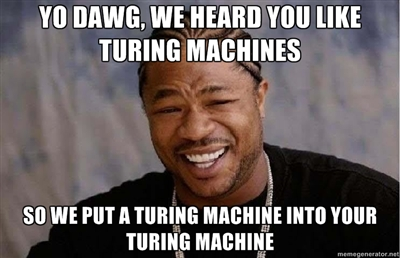
\includegraphics[scale=.5]{graphics/13/33928220.jpg}
   \end{figure}}
\end{frame}
\begin{frame}{Codierungen von Turingmaschinen: Gödelisierung}
    Wir codieren eine Turingmaschine so:
    \begin{itemize}
        \item Das Alphabet ist $\left\{ 0, 1, [, ] \right\}$.
            \pause
        \item Die Zustände werden durchnummeriert, Startzustand mit $0$, Zustände haben gleich viele Stellen, eingeklammert in $[]$. Dafür schreiben wir $\cod_z\left( Z \right)$.
            \pause
        \item Bandalphabet wird auch durchnummeriert, Blanket ist $0$. Dafür schreiben wir $\cod_x\left( x \right)$.
            \pause
        \item Bewegungsrichtungen werden mit $[10]$, $[00]$, $[01]$ codiert (links, stehen bleiben, rechts). Dafür schreiben wir $\cod_M\left( r \right)$.
        \item Auch die partiellen Funktionen $f$, $g$ und $m$ werden codiert. (Skript)
    \end{itemize}
    \pause
    Das ganze nennen wir \emph{Gödelisierung}. Jede Turingmaschine hat dann eine \emph{Gödelnummer}.
\end{frame}
\begin{frame}{Beispiel zur Gödelisierung}
Gegeben ist die Turingmaschine $T = \left( \left\{ z_0, z_1, z_2 \right\}, z_0, \left\{ \square, a, b, c, d \right\}, f, g, m \right)$. Codiert alles außer $f, g, m$.
    \begin{itemize}
        \visible<2->{\item $\cod_z\left( z_0 \right) = [00]$}
        \visible<3->{\item $\cod_z\left( z_1 \right) = [01]$
        \item $\cod_z\left( z_2 \right) = [10]$
        \item $\cod_x\left( \square \right) = [000]$
        \item $\cod_x\left( a \right) = [001]$
        \item $\cod_x\left( b \right) = [010]$
        \item $\cod_x\left( c \right) = [011]$
        \item $\cod_x\left( d \right) = [100]$}
    \end{itemize}
    Muss alles angegeben werden?\\
    \visible<4->{Nein, es reicht jeweils das größte Element.}
\end{frame}
\begin{frame}{Halteproblem-Beweis 1}
    \begin{block}{Satz}
        Es ist nicht möglich, eine Turingmaschine $U$ zu bauen, die für jede Turingmaschine $T$ (codiert als $w_1$) und jede Eingabe $w_2$  entscheidet, ob $T$ bei der Eingabe von $w_2$ hält.
    \end{block}
    Das lässt sich auch beweisen. 
\end{frame}
\begin{frame}{Beweis des Halteproblems}
    Annahme: es gibt eine Super-Turingmaschine $H$. $H$ bekommt als Eingabe:
    \begin{itemize}
        \item eine andere Turingmaschine $T$ und
        \item ein Eingabewort $w$.
    \end{itemize}
    \pause
    Die Super-Turingmaschine $H$ 
    \begin{itemize}
        \item simuliert die ``normale'' Turingmaschine $T$ und
        \item benutzt als Eingabe für $T$ das Wort $w$.
    \end{itemize}
    \pause
    Die Super-Turingmaschine $H$ gibt aus
    \begin{itemize}
        \item $1$, wenn $T$ mit $w$ als Eingabe hält und
        \item $0$, wenn $T$ mit $w$ als Eingabe nicht hält.
    \end{itemize}
\end{frame}
\begin{frame}{Halteproblem-Beweis 2}
    Wir bauen uns eine unendlich große Tabelle, die
    \begin{itemize}
        \item nach rechts (in den Spalten) alle möglichen Worte $w$ enthält und
        \item nach unten (in den Zeilen) die codierte Turingmaschine $T_w$ zum Wort $w$ enthält.
    \end{itemize}
    In den Zeilen sind also \emph{alle möglichen Turingmaschinen}.
    \pause
    Unsere Super-Turingmaschine hat die Tabelle ausgefüllt mit
    \begin{itemize}
        \item $1$, wenn $T_w\left( w \right)$ hält und
        \item $0$, wenn $T_w\left( w \right)$ nicht hält.
    \end{itemize}
    \pause
    \begin{table}
        \centering
        \begin{tabular}{ccccl}
            \toprule
                     & $w_0$ & $w_1$ & $w_2$ & \dots\\
             \midrule
             $T_{w_0}$ & 1 & 0 & 1 & \\
             $T_{w_1}$ & 0 & 0 & 0 & \\
             $T_{w_2}$ & 0 & 0 & 1 & \\
             \dots   &  &   &   &  \\
%             $T_d$ & 1 & 0 & 1 & ($\leftarrow$ das ist die Diagonale) \\
%             $T_{\overline{d}}$ & 0 & 1 & 0 & ($\leftarrow$ die Zeile war sicher noch nirgends) \\
             \bottomrule
        \end{tabular}
    \end{table}
\end{frame}
\begin{frame}{Halteproblem-Beweis 3}
    Nun nehmen wir die Diagonale und schreiben sie auch in die Tabelle (hier \textcolor{blue}{blau}). Außerdem schreiben wir darunter das ``Komplementär'' der Diagonale ($1$ wird zu $0$ und umgekehrt, hier in \textcolor{red}{rot}).
    \begin{table}
        \centering
        \begin{tabular}{ccccl}
            \toprule
                     & $w_0$ & $w_1$ & $w_2$ & \dots\\
             \midrule
             $T_{w_0}$ & \textcolor{blue}{1} & 0 & 1 & \dots\\
             $T_{w_1}$ & 0 & \textcolor{blue}{0} & 0 & \dots\\
             $T_{w_2}$ & 0 & 0 & \textcolor{blue}{1} & \dots\\
             \dots   &  \dots & \dots  & \dots  & \dots \\
             $T_d$ & \textcolor{blue}{1} & \textcolor{blue}{0} & \textcolor{blue}{1} &\dots ($\leftarrow$ das ist die Diagonale) \\
             $T_{\overline{d}}$ & \textcolor{red}{0} & \textcolor{red}{1} & \textcolor{red}{0} & \dots($\leftarrow$ die Zeile war sicher noch nirgends) \\
             \bottomrule
        \end{tabular}
    \end{table}
    Warum gibt es $T_{\overline{d}}$ nicht schon vorher?\\
    \visible<2->{Sie unterscheidet sich von jeder Zeile um ein Element (Diagonalelement).}
\end{frame}
\begin{frame}{Halteproblem-Beweis 4}
    \begin{table}
        \centering
        \begin{tabular}{ccccl}
            \toprule
                     & $w_0$ & $w_1$ & $w_2$ & \dots\\
             \midrule
             $T_{w_0}$ & \textcolor{blue}{1} & 0 & 1 & \dots\\
             $T_{w_1}$ & 0 & \textcolor{blue}{0} & 0 & \dots\\
             $T_{w_2}$ & 0 & 0 & \textcolor{blue}{1} & \dots\\
             \dots   &  \dots & \dots  & \dots  & \dots \\
             $T_d$ & \textcolor{blue}{1} & \textcolor{blue}{0} & \textcolor{blue}{1} &\dots ($\leftarrow$ die Zeile war schon irgendwo) \\
             $T_{\overline{d}}$ & \textcolor{red}{0} & \textcolor{red}{1} & \textcolor{red}{0} & \dots($\leftarrow$ die Zeile war sicher noch nirgends) \\
             \bottomrule
        \end{tabular}
    \end{table}
    Obwohl $T_{\overline{d}}$ sicher nirgends vorkam, könnten wir sie bauen:
    \begin{itemize}
        \item Wir wissen, dass $T_d$ hält (sagt uns die Super-Turingmaschine), also gehen wir mit $T_{\overline{d}}$ in eine Endlosschleife.
        \item Wir wissen, dass $T_d$ nicht hält (sagt uns die Super-Turingmaschine), also halten wir mit $T_{\overline{d}}$.
    \end{itemize}
    \pause
    Verrückt: Wenn es die Super-Turingmaschine gibt, dann könnten wir die Turing-Maschine $T_{\overline{d}}$ bauen, die es eigentlich nicht gibt. Das ist ein Widerspruch, also kann es die Super-Turingmaschine nicht geben.
\end{frame}
\begin{frame}{Die Busy-Beaver-Funktion}
    \begin{block}{Definition: Busy-Beaver-Funktion}
        Der Busy-Beaver (``fleißiger Biber'') ist eine Turingmaschine, die $n+1$ Zustände, wobei ein Anfangszustand und ein Haltezustand darunter sind. Diese Turingmaschine kann nur $1$ auf das Band schreiben.\\
        Die Busy-Beaver-Funktion $\mathrm{bb}\left( n \right)$ wird der fleißige Biber genannt, der die maximale Anzahl an Einsen auf das Band schreiben kann (also der fleißigste Biber).
    \end{block}
    \pause
    \begin{block}{Theorem}
        Für jede berechenbare Funktion $f: \mathbb{N}_+ \rightarrow \mathbb{N}_+$ gibt es ein $n_0$, so dass für alle $n \geq n_0$ gilt:
        \begin{align*}
            \mathrm{bb}\left( n \right) > f(n)
        \end{align*}
    \end{block}
    Kurz: Die Busy-Beaver-Funktion ist die am schnellsten wachsende Funktion. Und nicht berechenbar.
\end{frame}
\begin{frame}{Beispiel zum Busy-Beaver}
    Wie viele Einsen produziert diese Turingmaschine? Übrigens: Das ist $\mathrm{bb}\left( 4 \right)$.
    \begin{table}
        \centering
        \begin{tabular}{cccccc}
            \toprule
             & A & B & C & D & H\\
             \midrule
             \sq & $1, R, B$ & $1, L, A$ & $1, R, H$ & $1, R, D$ & \\
             $1$ & $1, L, B$ & \sq$ , L, C$ & $1, L, D$ & \sq$ , R, A$ & \\
            \bottomrule
        \end{tabular}
    \end{table}
    \visible<2->{Diese Turingmaschine produziert 13 Einsen.}
\end{frame}
\section{Äquivalenzrelationen}
\begin{frame}{Äquivalenzrelation}
    \begin{block}{Definition: Äquivalenzrelation}
        Eine Relation $R$ ist genau dann eine \emph{Äquivalenzrelation}, wenn sie
        \begin{itemize}
            \item symmetrisch,
            \item reflexiv und
            \item transitiv
        \end{itemize} ist.
    \end{block}
\end{frame}
\begin{frame}{Eigenschaften von Relationen}
    Welche Eigenschaften haben diese Relationen (stets auf ganze Zahlen)?
    \begin{itemize}
        \item $\leq$ \visible<2->{reflexiv, transitiv}
        \item $>$ \visible<3->{transitiv}
        \item $=$ \visible<4->{reflexiv, transitiv, symmetrisch}
    \end{itemize}
    Wie sieht das in einem Graphen aus? (Tafel)\\
    \pause
    Könnt ihr euch noch weitere Äquivalenzrelationen vorstellen? \visible<5->{(Denkt an Betrag, die Quersumme, Modulo)}
\end{frame}
\begin{frame}{Äquivalenzrelation Kongruenz Modulo}
    \begin{block}{Definition: Kongruent Modulo}
        Zwei Zahlen $x, y\in \mathbb{N}_+$ heißen \emph{kongruent modulo n}, wenn die Differenz $x-y$ durch $n$ teilbar, also ein Vielfaches von $n$ ist. Es wird geschrieben:
        \begin{align*}
            x \equiv y \left( \mod n \right)
        \end{align*}
    \end{block}
    Beweis (Auszug):
    \visible<2->{\begin{itemize}
        \item Reflexivität: $x-x = 0$ ist Vielfaches von $n$.
            \pause
        \item Symmetrie: $x-y$ ist Vielfaches von $n$, $\Rightarrow y-x = -\left( x-y \right)$ ist auch Vielfaches von $n$
            \pause
        \item Transitivität: $x-y = k_1 n$ und $y-z = k_2 n$ ($k_1, k_2 \in \mathbb{Z}$), dannn ist\\
            $x-z = (x-y) + (y-z) = (k_1 + k_2)\cdot n$ ein Vielfaches von n.
    \end{itemize}}
\end{frame}
\begin{frame}{Äquivalenzklasse}
    \begin{block}{Definition: Äquivalenzklasse}
        Sind zwei Elemente $\left( x,y \right)\in R$, so schreibt man auch $xRy$ (Infixschreibweise). Alle Elemente, die miteinander in Relation stehen, befinden sich in der selben \emph{Äquivalenzklasse}:
        \begin{align*}
            [x]_\mathrm{R} = \left\{ y | yRx \right\}
        \end{align*}
    \end{block}
\end{frame}
\begin{frame}{Quiz}
    \begin{itemize}
        \item Stimmt es, dass auch $xRy$ folgt: $[x]_\mathrm{R} = [y]_{\mathrm{R}}$? \visible<2->{Ja.}
        \item Existiert ein $z\in \left[ x \right]_\mathrm{R}$ und $z\in\left[ y \right]_\mathrm{R}$, so ist $\left[ x \right]_\mathrm{R} = \left[ y \right]_\mathrm{R}$. \visible<3->{Ja.}
        \item Wieviele Äquivalenzklassen gibt es zu $R = \mod 6$? \visible<4->{6}
    \end{itemize}
\end{frame}
\begin{frame}{Nerode-Äquivalenzrelation}
    \begin{block}{Definition: Nerode-Äquivalenzrelation}
        Sei $L\subseteq A^*$ eine formale Sprache. $w_1$ und $w_2$ seien Wörter $\in A^*$. Die Wörter heißen \emph{Nerode-Äquivalent} ($\equiv_L$), falls gilt:
        \begin{align*}
            w_1 \equiv_L w_2 \Leftrightarrow \left( \forall w \in A^*: w_1 w\in L \leftrightarrow w_2 w\in L \right)
        \end{align*}
    \end{block}
\end{frame}
\begin{frame}{Beispiel zur Nerode Äquivalenz}
    \begin{itemize}
        \item Alphabet $A = \left\{ a,b \right\}$
        \item Sprache $L \subset A*$, $L$ enthält alle Wörter ohne das Teilwort $ba$: $L = \left< a^* b^*\right>$
    \end{itemize}
    Wie sieht der zugehörige Automat aus?
    \begin{columns}
        \begin{column}{.5\textwidth}
            \visible<2->{\begin{figure}
                \centering
                \begin{tikzpicture}[shorten >=1pt,initial text=,node distance=2cm,auto,->,>=stealth]
                    \node[state,initial,accepting]  (1)                    {1};
                    \node[state,accepting]  (2)[right of=1]        {2};
                    \node[state]  (J)[below right of=1]  {J};

                    \path[->]
                        (1) edge              node  {b} (2)
                        (1) edge [loop above] node  {a} ()
                        (2) edge [loop above] node  {b} ()
                        (2) edge              node  {a} (J)
                        (J) edge [loop below] node  {a,b} ()
                    ;
                \end{tikzpicture}
            \end{figure}}
        \end{column}
        \begin{column}{.5\textwidth}
            \visible<3->{Wie kann jeder Zustand erreicht werden?}
            \visible<4->{\begin{itemize}
                \item $a^*$
                \item $a^*bb^*$
                \item $a^*bb^*a\left\{ a,b \right\}^*$
            \end{itemize}}
            Nerode-Äquivalenzklassen: $\visible<5->{\left[ \epsilon \right], \left[ b \right], \left[ ba \right]$.}
        \end{column}
    \end{columns}
\end{frame}
\begin{frame}{Faktormenge}
    \begin{block}{Definition: Faktormenge}
        Die Menge aller Äquivalenzklassen einer Menge zur Relation $R$ bezeichnet man als \emph{Faktormenge} und schreibt $M_\mathrm{/R}$.
    \end{block}
\end{frame}
\begin{frame}{Beispiel zur Faktormenge}
    \begin{itemize}
        \item Nennt die Äquivalenzklassen zu Kongruenz modulo $5$. (Natürlich auf ganzen Zahlen.)\\
            \visible<2->{$[0], [1], [2], [3], [4]$}
        \item Nennt die Faktormenge dazu.\\
            \visible<3->{$\mathbb{Z}_{/\equiv_5} = \left\{ [0], [1], [2], [3], [4] \right\}$}
    \end{itemize}
\end{frame}
\begin{frame}{Beispiel 2 zur Nerode-Äquivalenz}
    Gegeben sei die Sprache $L = \left\{ a^k b^k | k \in \mathbb{N}_0 \right\}$. \\
    Wie sieht hier ein endlicher Akzeptor aus?
    \visible<2->{Es gibt keinen.}\\
    \visible<3->{Nennt einige Nerode-Äquivalenzklassen.}\\
    \visible<4->{Wieviele gibt es?}\\
    \visible<5->{Es gibt unendlich viele Nerode-Äquivalenzklassen. Die Faktormenge hat also unendlich viele Elemente.}
\end{frame}
\begin{frame}{}
    
\includegraphics[scale=.40]{graphics/13/timetraveler4.png}\\
    http://www.explosm.net/comics/1633/
\end{frame}
\end{document}
